\documentclass[12pt]{article}

\usepackage{pdfsync}
\usepackage{amsmath}
\usepackage{graphicx}

\graphicspath{{./figures/}}

%%%%%%%%%%%%%%%%%%%%%%%%%%%%%%%%%%%%%%%%%%%%%%%%%%%%%%%%%%%%
\renewcommand{\d}{\mathrm{d}}
\newcommand{\vv}[1]{\boldsymbol{#1}}
\newcommand{\cB}{B}
\newcommand{\cA}{A}
\newcommand{\cC}{C}


%%%%%%%%%%%%%%%%%%%%%%%%%%%%%%%%%%%%%%%%%%%%%%%%%%%%%%%%%%%%


\begin{document}

\section{Active Flagella}\label{active-flagella}

We mimic the formulation in \cite{CamaletJulicher2000}, with a
discretization in weak form, and with a spontaneous curvature, instead
of the internal force.

\subsection{Formulation of the energy}\label{formulation-of-the-energy}

Given a configuration \(X(s)\) of an active filament, its energy can be expressed by

\[G(X) = \int_0^L \left( \frac{\cB}{2}(\kappa-\alpha)^2 +
  \frac{\Lambda}{2} X_s^2 \right) \d s\]

Where $\alpha$ is an \emph{active curvature}, $\cB$ is an \emph{active
  bending modulus}, $\kappa$ is the \emph{curvature}, $s$ is the
\emph{arclength}, while $\Lambda$ is the \emph{Lagrange multiplier}
associated with the constraint $X_s^2 = 1$.

For a two dimensional curve parametrized by arclength, we can define
the tangent vector $t = X_s$ as $t = (\cos(\theta), \sin(\theta))$, and
we can define all quantities of interest in terms of $\theta$. For
example, $t_s = \kappa n$, $n_s = -\kappa t$ and $\kappa = \theta_s$.

Once a function defining \(\theta(s)\) is available, we can reconstruct
the position of the curve as

\[X(s) = X_0 + \int_0^s \left(\cos(\theta(s'), \sin(\theta(s') \right)
\d s'\]

We can model the internal forces generated by the active curvature
$\alpha$ and the active bending modulus $\cB$ as

\[f_e = -\frac{\partial G}{\partial X} = (\eta n + \tau t)_s\]

Where \(\eta\) is the \emph{shear}, while $\tau$ is the
\emph{tension}. Given 

\[\zeta := -\cB(\kappa - \alpha) = -\cB(\theta_s - \alpha)\]

we can write the shear as

\[\eta := \zeta_s := -\big( \cB(\kappa - \alpha) \big)_s\]

and the tension as:

\[\tau := -\zeta\kappa + \Lambda = \cB(\theta_s-\alpha)\kappa +\Lambda\]

\subsection{Resistive force theory}
\label{sec:resist-force-theory}



When immersed in a fluid, if we use \emph{resistive force theory},
then the force applied by fluid on the filament can be modeled as

\[f_f = -( \xi_\perp n\otimes n +\xi_\parallel t\otimes t) X_t\]

that is

\[X_t = -\left( \frac{1}{\xi_\perp}  n\otimes n + \frac{1}{\xi_\parallel} t\otimes t\right) f_f\]

From equilibrium, we have

\[f_e+f_f = 0\]

that is

\[X_t = \left( \frac{1}{\xi_\perp}  n\otimes n + \frac{1}{\xi_\parallel} t\otimes t\right) (\eta n + \tau t)_s\]

Exploiting the fact that \(n_s = - \kappa t\) and \(t_s = \kappa n\), we
arrive at

\[X_t =  \frac{1}{\xi_\perp} (\eta_s + \kappa \tau) n + \frac{1}{\xi_\parallel}(\tau_s - \kappa \eta) t\]

Writing $\gamma = \frac{\xi_\perp}{\xi_\parallel}$, we obtain:

\[\xi_\perp X_t =   (\eta_s + \kappa \tau) n + \gamma (\tau_s - \kappa \eta) t\]

\subsection{Excluding the Lagrange multiplier}\label{differential-derivation}

We know from the reconstruction of the curve that
\(X_{ts} = X_{st} = \theta_s n\),
and we can exploit this to obtain two equations involving only
\(\theta\),
\(\eta\)
and \(\tau\) (here written also in term of $\kappa = \theta_s$):

\[ \xi_\perp X_{ts}\cdot n =\xi_\perp \theta_t =   (\eta_s + \kappa \tau)_s + \gamma (\kappa \tau_s - \kappa^2 \eta)\]

\[X_{ts}\cdot t = 0 =  \gamma(\tau_s - \kappa \eta)_s - (\kappa \eta_s + \kappa^2 \tau) \]

We linearize this system by splitting all nonlinear terms (which are
only nonlinear because they contain \(\kappa\)), and by iterating over
\(\theta\) until convergence, and constructing \(\bar\kappa\) of the
previous iteration. If we introduce three independent variables
\(\theta\), \(\eta\) and \(\tau\), for any \(\bar\kappa\), we can write
the linear system:

\[\begin{pmatrix}
-(B\theta_s)_s & -\eta &  \\
%%
%%
\xi_\perp\theta_t & 
-\eta_{ss} + \gamma \bar \kappa^2\eta &
- (\bar\kappa\tau)_s - \gamma\bar\kappa\tau_s \\
%%
%%
 & 
\bar \kappa\eta_s +\gamma(\bar \kappa\eta)_s &
 - \gamma\tau_{ss} + \bar \kappa^2 \tau
\end{pmatrix}
%
=
\begin{pmatrix}
-(B\alpha)_s\\
0\\
0
\end{pmatrix}\]

We multiply the three equations by test functions
$(\delta \theta, \delta\eta, \delta \tau)$, and we integrate by parts
whenever it is convenient. We adopt the following notation:
\[
(a,b) := \int_0^1 a(s) b(s) \d s
\]
\[
\langle a,b \rangle := a(s) b(s) \big|^1_0 = a(1)b(1)-a(0)b(0),
\]
and we move all known terms and boundary terms on the right hand side:

\begin{multline}
\begin{pmatrix}
(B\theta_s, \delta \theta_s)  &  -(\eta,\delta\theta)  & 0 \\
%%
%%
\xi_\perp(\theta_t, \delta \eta) & 
(\eta_{s}, \delta \eta_s) 
+ \gamma (\bar \kappa^2\eta, \delta\eta) &
 (\bar\kappa\tau, \delta\eta_s) 
- \gamma(\bar\kappa\tau_s, \delta\eta) \\
%%
%%
0 & 
(\bar \kappa\tau_s, \delta\tau) 
-\gamma(\bar \kappa\eta, \delta\tau_s) &
%
%
+ \gamma(\tau_{s},\delta\tau_s) 
+ (\bar \kappa^2 \tau, \delta\tau)
\end{pmatrix}
%
\\
=
\begin{pmatrix}
(B\alpha, \delta \theta_s)& +\langle B(\theta_s-\alpha), \delta \theta\rangle\\
& \langle \eta_s+\bar\kappa\tau,\delta\eta\rangle
\\
&\gamma\langle\tau_{s}-\bar \kappa\eta, \delta\tau\rangle 
\end{pmatrix}
\end{multline}

\subsection{Discretization}

For the three fields $\theta, \eta$ and $\tau$, we introduce the
following spaces:

\begin{equation}
  \label{eq:1}
    V^a_{0/1}  = \{ a \in H^m([0,1])^3 \text{ s.t. } a(0/1) = 0\},
\end{equation}
%
where the superscript $a$ is either $\theta$, $\eta$ or $\tau$, while
the subscript $0$ or $1$ means that functions in this space are zero
on $s=0$ or $s=1$.

Except from the boundary conditions, we use the same basis functions
to discretize both $(\theta, \eta, \tau)$ and $(\delta\theta, \delta
\eta, \delta \tau)$. In particular, the discrete spaces can be written
as 
\begin{equation}
  \label{eq:3}
  V_h := \text{span} \{ N_i(s) \}_{i=1}^n
\end{equation}
and any function $v$ in $V_h$ can be written as
$$
v(s)  = v^i N_i(s)
$$
where we use Einstein summation convention.


\subsection{Matrix form of the weak
formulation}\label{matrix-form-of-the-weak-formulation}

Given an arbitrary field \(\gamma\),
we'll use the following shorthand notation:

\begin{equation}
  \label{eq:2}
  \begin{aligned}
    \vv A^\gamma_{ij} & = (\gamma N_j', N_i') &  = \int_0^1 \gamma(s) N_j'(s)
    N_i'(s) \d s \\
    \vv B^\gamma_{ij} & = (\gamma N_j', N_i) & = \int_0^1 \gamma(s) N_j'(s)
    N_i(s) \d s \\
    \vv M^\gamma_{ij} & = (\gamma N_j, N_i) & = \int_0^1 \gamma(s) N_j(s)
    N_i(s) \d s 
  \end{aligned}
\end{equation}

If we restrict the functions $\theta, \eta, \tau$ to live in $V_h$, we
can rewrite the system above in matrix form:


\begin{multline}
\label{eq:4}
\xi_\perp\vv M \theta_t + 
\begin{pmatrix}
\vv A^B &  -\vv M & 0 \\
%%
%%
0 & 
 \vv A
+ \gamma \vv M^{\bar \kappa^2} &
 \vv B^{\bar\kappa T}
- \gamma\vv B^{\bar\kappa} \\
%%
%%
0 & 
 \vv B^{\bar\kappa}
- \gamma\vv B^{\bar\kappa T} 
&
%
%
\gamma \vv A
+ \vv M^{\bar \kappa^2}
\end{pmatrix}
%
\begin{pmatrix}
\theta\phantom{\big|\!\!}\\
\eta\phantom{\big|\!\!} \\
\tau\phantom{\big|\!\!}
\end{pmatrix}
=\\
\begin{pmatrix}
\vv B^{BT}\alpha & +\langle B(\theta_s-\alpha), \delta \theta\rangle\\
& \langle \eta_s+\bar\kappa\tau,\delta\eta\rangle
\\
&\gamma\langle\tau_{s}-\bar \kappa\eta, \delta\tau\rangle 
\end{pmatrix}
\end{multline}

The simplest possible discretization (IMEX with Explicit euler for
nonlinear terms and implicit euler for linear ones) is obtained by
setting
$$
\theta_t = \frac{\theta^{k+1} - \theta^k}{dt} \qquad k \in
[1,2,3,\ldots, N_t], \qquad \theta^0 \text{ given}
$$
and inserting in $\bar \kappa$ the curvature of the previous time step
$\bar \kappa := \theta^k_s$, that is, we solve the problem:

Given $dt, B, \alpha$ and $\theta^k, \bar \kappa = \theta^k_s$, find
$\theta^{k+1}$, $\eta^{k+1}$ and $\tau^{k+1}$ as the solution to

\begin{multline}
\label{eq:4}
\begin{pmatrix}
\vv A^B &  -\vv M & 0 \\
%%
%%
\frac{1}{dt} \vv M& 
 \vv A
+ \gamma \vv M^{\bar \kappa^2} &
 \vv B^{\bar\kappa T}
- \gamma\vv B^{\bar\kappa} \\
%%
%%
0 & 
 \vv B^{\bar\kappa}
- \gamma\vv B^{\bar\kappa T} 
&
%
%
\gamma \vv A
+ \vv M^{\bar \kappa^2}
\end{pmatrix}
%
\begin{pmatrix}
\theta^{k+1}\phantom{\big|\!\!}\\
\eta^{k+1}\phantom{\big|\!\!} \\
\tau^{k+1}\phantom{\big|\!\!}
\end{pmatrix}
=\\
\begin{pmatrix}
\vv B^{BT}\alpha & +\langle B(\theta_s-\alpha), \delta \theta\rangle\\
\frac{1}{dt} \vv M \theta^k& +\langle \eta_s+\bar\kappa\tau,\delta\eta\rangle
\\
&\gamma\langle\tau_{s}-\bar \kappa\eta, \delta\tau\rangle 
\end{pmatrix}
\end{multline}

\subsection{Small deformations}\label{small-deformations}

We perform a systematic expansion of the filament dynamics in powers of the dimensionless amplitude \epsilon by writing

$$
\begin{aligned}
\theta = \epsilon\theta_1 \\
\eta = \epsilon\eta_1 \\
\tau = \tau_0 + \epsilon^2 \tau_2 \\
\alpha = \epsilon \alpha_1
\end{aligned}
$$

Proceding exactly in the same way as done for the nonlinear problem, we solve the linear problem:\\
Given $dt, B, \alpha, \theta^k, \theta^k_s$, and $\sigma$ find
$\theta^{k+1}$ and $\eta^{k+1}$ as the solution to

\begin{multline}

\begin{pmatrix}
\vv A^B &  -\vv M  \\
%%
%%
\frac{1}{dt} \vv M + \vv A^\sigma & \vv A \\
%%
%%
\end{pmatrix}
%
\begin{pmatrix}
\theta^{k+1}\phantom{\big|\!\!}\\
\eta^{k+1}\phantom{\big|\!\!} 
\end{pmatrix}
=\\
\begin{pmatrix}
\vv B^{BT}\alpha & +\langle B\theta_s, \delta \theta\rangle\\
\frac{1}{dt} \vv M \theta^k& +\sigma \langle \theta_s+\eta_s,\delta\eta\rangle
\end{pmatrix}
\end{multline}


\subsection{Boundary conditions}\label{boundary-conditions}

\begin{tabular}{l|c|c|c|c||c|c|c|}
  Type & BC on $\theta(0)$ & BC on $\eta(0)$ & BC on $\tau(0)$ & BC on $\theta(1)$ & BC on $\eta(1)$ & BC on $\tau(1)$ \\
  A & $\theta = 0$ & $v_n = 0$ & $v_t=0$ & $\zeta = 0$ &  $\eta = 0$& $\tau = 0$  \\
  B & $\zeta = 0$ & $v_n = 0$ & $v_t=0$  & $\zeta = 0$&  $\eta = 0$& $\tau = 0$ \\
  C &  $\zeta = 0$ & $\eta = -C v_n$& $\tau =  -C v_t$ & $\zeta = 0$&  $\eta = 0$& $\tau = 0$ \\
  D  &  $\theta = 0$ & $v_n = 0$& $v_t=0$ & $\zeta = 0$& $\eta \neq 0$& $\tau \neq 0$ 
\end{tabular}


\begin{itemize}
\item A: Clamped Head, free tail
\item B: Fixed Head, free tail
\item C: Swimming flagellum with viscous load 
\item D: clamped head, external force applied to tail
\end{itemize}

The two scalar conditions on $v_n$ and $v_t$, are a shorthand notation for

$$
\begin{aligned}
v_n = \eta_s + \kappa \tau = & 0 \\
v_t = \tau_s - \kappa \eta = & 0
\end{aligned}
$$

The condition of zero external forces, $F_{ext} = 0$, implies the two scalar conditions

$$
\begin{aligned}
\eta = &0 \\
\tau = &0
\end{aligned}
$$

while zero external torque, $T_{ext} = 0$, is equivalent to 

$$
\zeta = -B(\kappa-\alpha) = 0
$$

\subsubsection{Differential interpretation of the boundary
conditions}\label{differential-interpretation-of-the-boundary-conditions}

When we write \(X_t = 0\), we are using this as a shorthand notation for

\[X_t =  (\eta_s + \kappa \tau) n + \gamma(\tau_s - \kappa \eta) t = 0\]
%
that is, the two scalar conditions

\[\begin{aligned}
\eta_s + \kappa \tau = &0 \\
\tau_s - \kappa \eta = &0
\end{aligned}\]
%
which are homogeneous Neumann conditions for the spaces of $\eta$ and $\tau$.

Similarly, the condition \(F_{ext} = 0\) implies the two scalar
conditions

\[\begin{aligned}
\eta = &0 \\
\tau = &0
\end{aligned}\]
%
which are homogeneous Dirichlet conditions for the spaces of $\eta$
and $\tau$, while \(T_{ext} = 0\) is equivalent to

\[\zeta = -B(\kappa-\alpha) = 0\]
%
which is a homogeneous Neumann condition for the space of $\theta$. 

In case A of the boundary condition table, all boundary condition
terms in the right hand side of Equation~(\ref{eq:4}) are zero, either
because the test function is zero or because the Neumann boundary
condition is zero. 

\subsection{Circle test}\label{circle-test}

We work in a non-dimensionalized setting, that is, we assume that the
length of the filament is equal to one. We start with a simple test in
which the spontaneous curvature of our curve is constantly equal to
$2\pi$. In the rest position, this generates a circle. We start with
$\theta$ equal to zero everywhere (a straight filament), and we let it
evolve for a while. Figure~\ref{fig:circle-clamped} presents a few
snapshots of the curve evolution in time, for the clamped boundary
condition, while

\begin{figure}
  \centering
  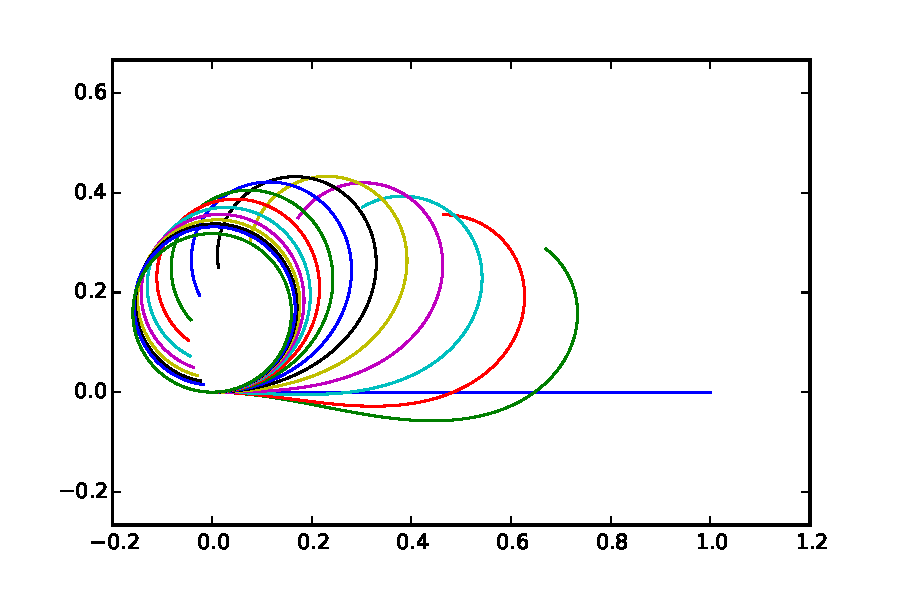
\includegraphics[width=\textwidth]{circle_clamped}
  \caption{Evolution of flat filament with constant spontaneous
    curvature. Clamped head.}
  \label{fig:circle-clamped}
\end{figure}

\begin{figure}
  \centering
  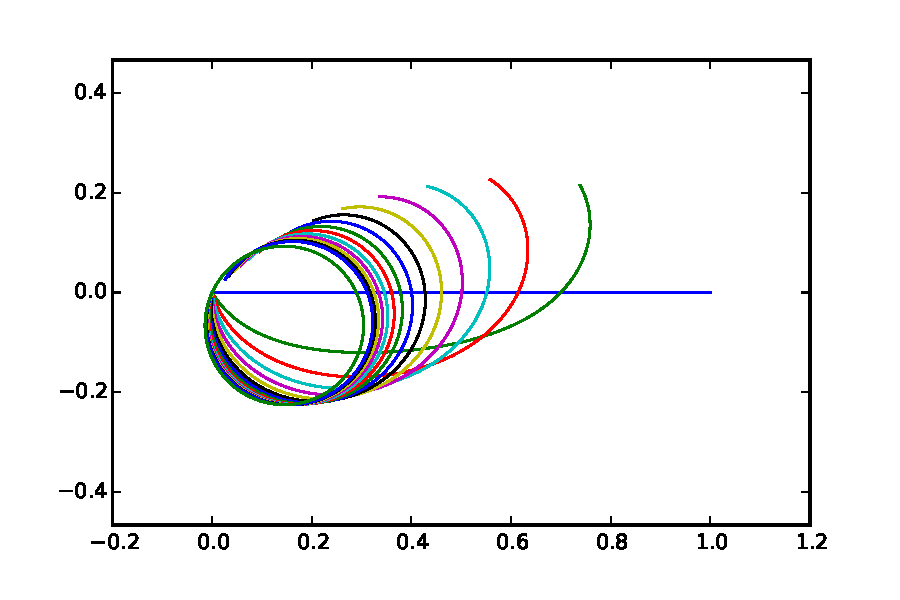
\includegraphics[width=\textwidth]{circle_pivoting}
  \caption{Evolution of flat filament with constant spontaneous
    curvature. Pivoting head.}
  \label{fig:circle-pivoting}
\end{figure}

\section{J\"ulicher formulation of the internal stress}

According to~\cite{CamaletJulicher2000} a filmanet motion can be expressed in terms of the reciprocal motion of microtubules.

There, the filament is thought to be composed of two sliding filaments, with configurations given by:

$$
\begin{aligned}
X_1(s) &= X(s)-a\frac{n(s)}{2} \\
X_2(s) &= X(s)+a\frac{n(s)}{2} 
\end{aligned}
$$
%
where $X$ is the position of the center line, and $a$ is the thickness of the filament. 
The sliding displacement at position $s$ along the neutral line $X$ is coupled with the curvature $\kappa$ as

$$
\Delta(s) = \int_0^s\left(|\partial_s X_1(s')|-|\partial_s
  X_2(s')|\right) \d s' = a\int_0^s \kappa(s') \d s'.
$$

If we introduce the force per unit length $f(s)$ acting at position
$s$ in opposite directions on the two microtubules, it can be shown
that the spontaneous curvature $\alpha(s)$ of the filament is related
to $f(s)$ from the following relations. Defining $F(s)$ as:

$$
F(s) := -\int_s^L f(s') ds'
$$

we have

$$
\alpha = a \frac{F(s)}{B}
$$

We consider the set of examples explored in~\cite{Gadelha2010}, where
$f(s)$ is assumed to be a simple travelling wave:

$$
f(s,t) = A \cos(\omega s - 2\pi t).
$$

They express everything in terms of $\omega$ and of the \emph{Sperm
  Compliance} $Sp$, defined (with our notations) as

$$
Sp := \left(\frac{2\pi \xi_\perp}{B}\right)^{\frac{1}{4}}.
$$

\begin{figure}
  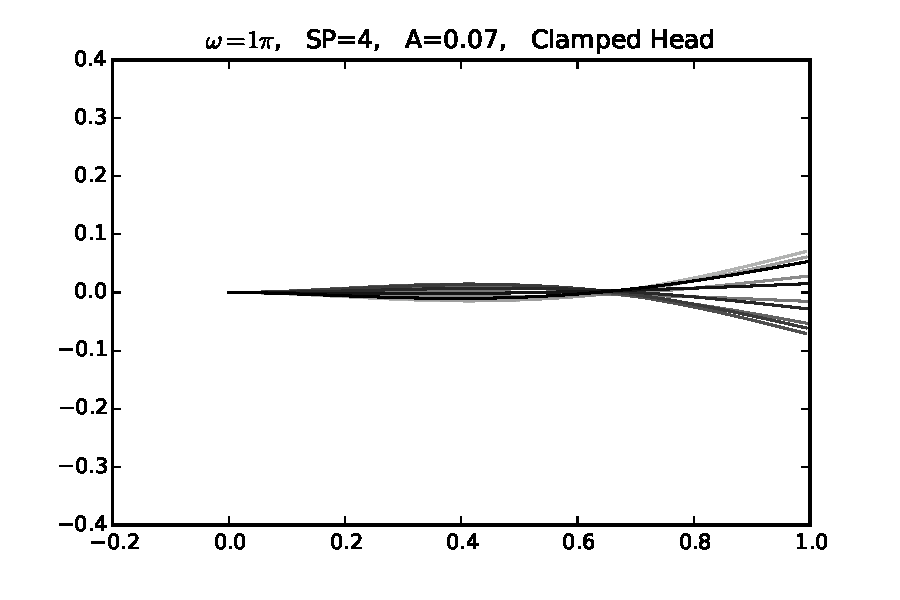
\includegraphics[width=.3\textwidth]{clamped_4_1}
  \hfill
  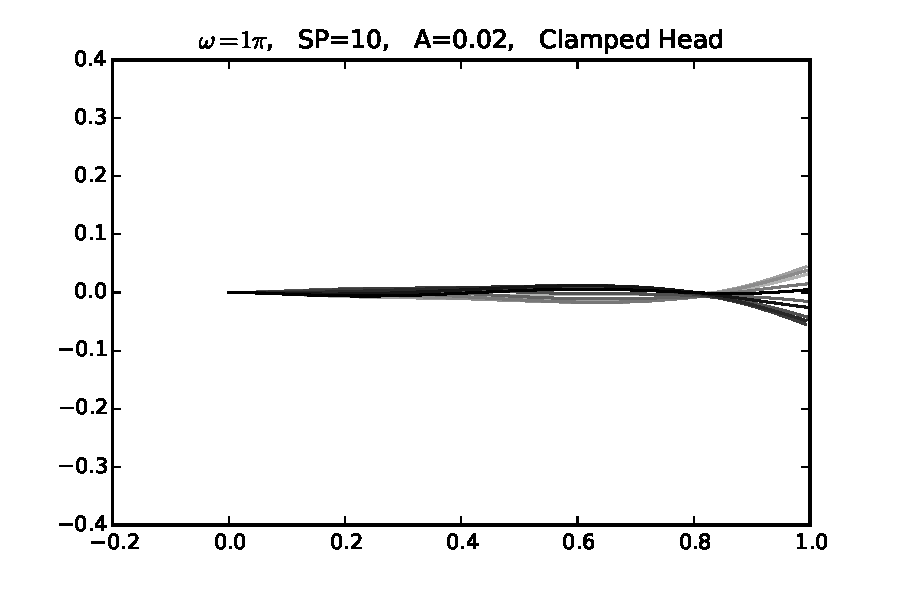
\includegraphics[width=.3\textwidth]{clamped_10_1}
  \hfill
  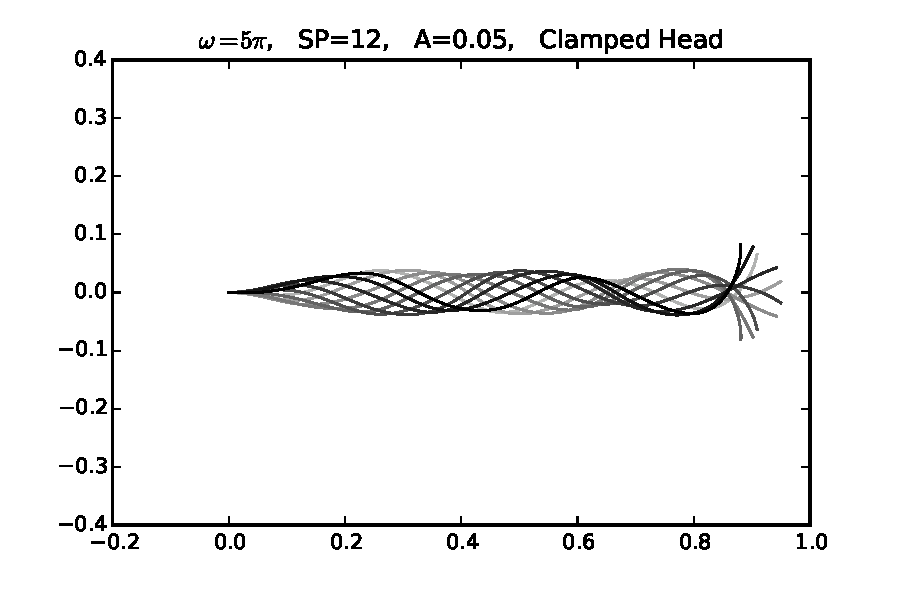
\includegraphics[width=.3\textwidth]{clamped_12_5}
  
  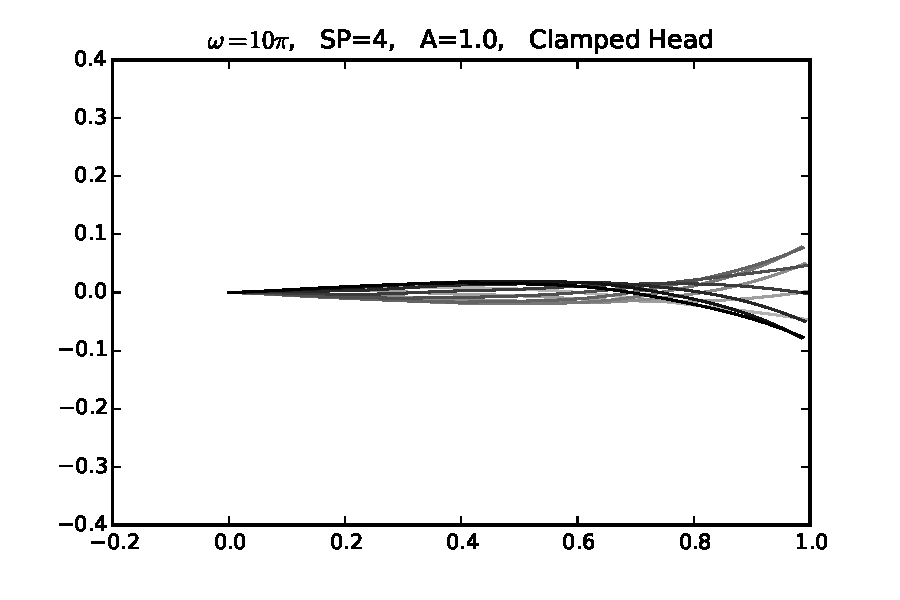
\includegraphics[width=.3\textwidth]{clamped_4_10}
  \hfill
  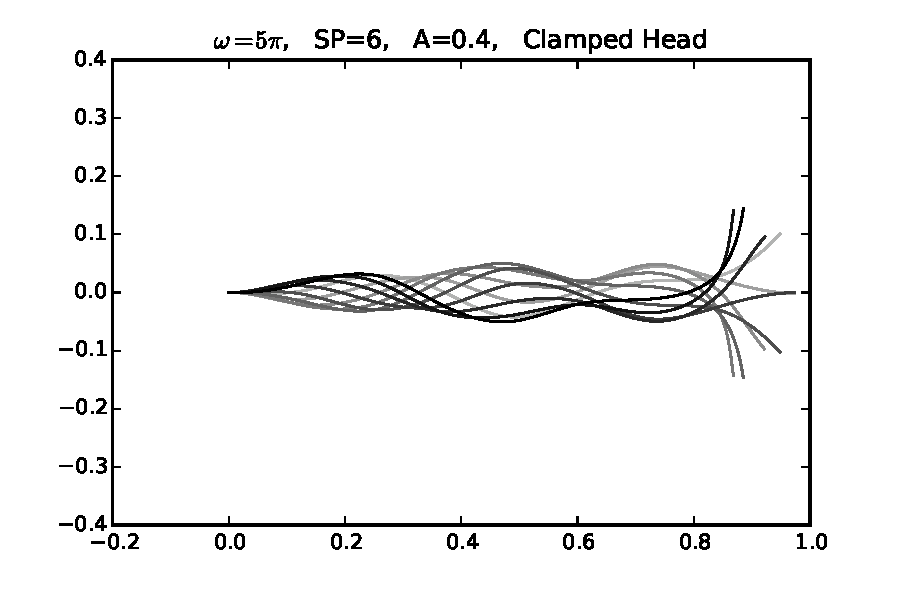
\includegraphics[width=.3\textwidth]{clamped_6_5}
  \hfill
  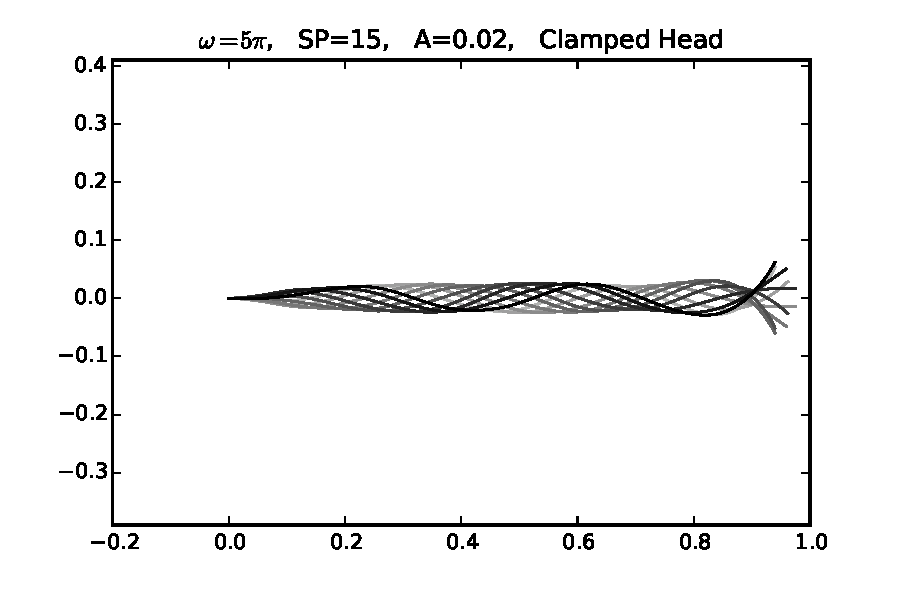
\includegraphics[width=.3\textwidth]{clamped_15_5}


  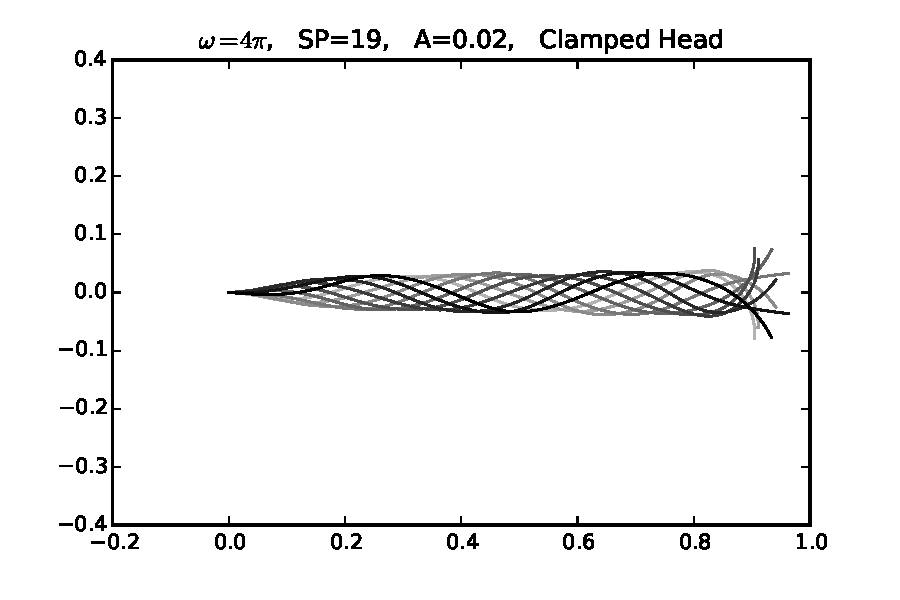
\includegraphics[width=.3\textwidth]{clamped_19_4}
  \hfill
  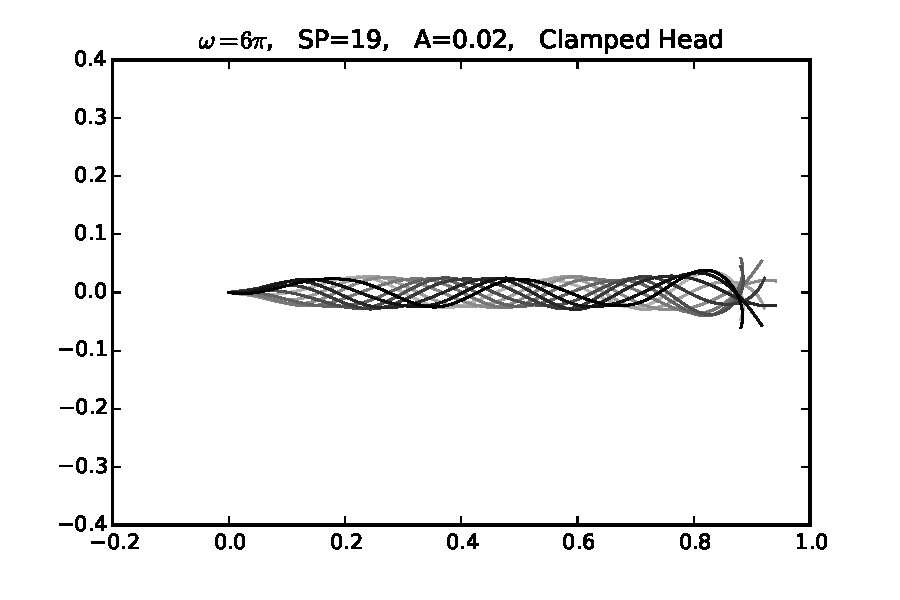
\includegraphics[width=.3\textwidth]{clamped_19_6}
  \hfill
  \includegraphics[width=.3\textwidth]{clamped_19_9}



  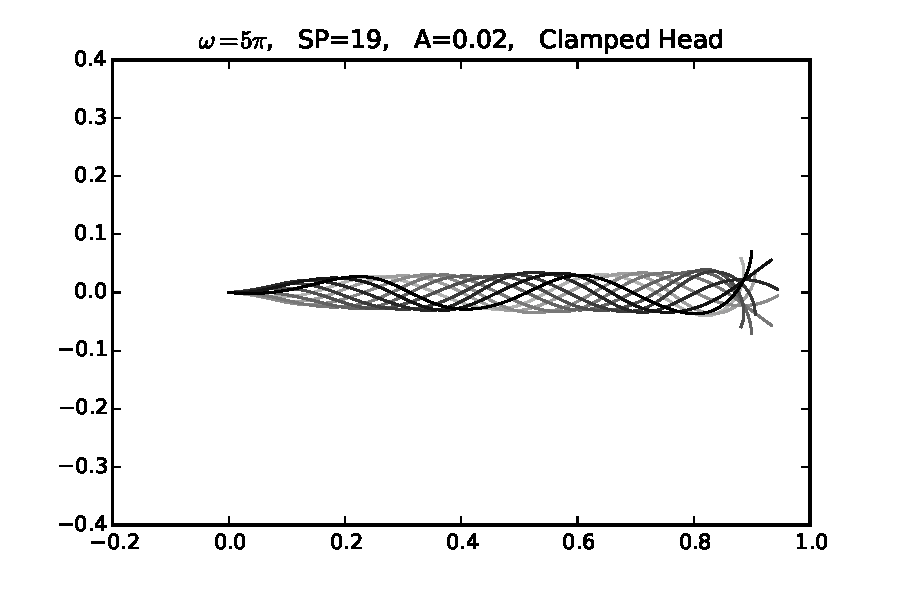
\includegraphics[width=.3\textwidth]{clamped_19_5}
  \hfill
  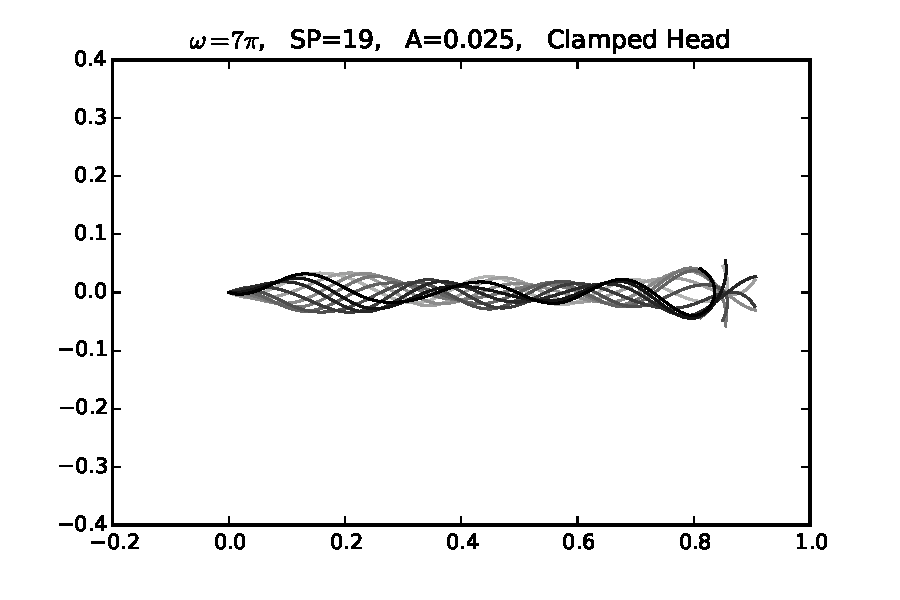
\includegraphics[width=.3\textwidth]{clamped_19_7}
  \hfill
  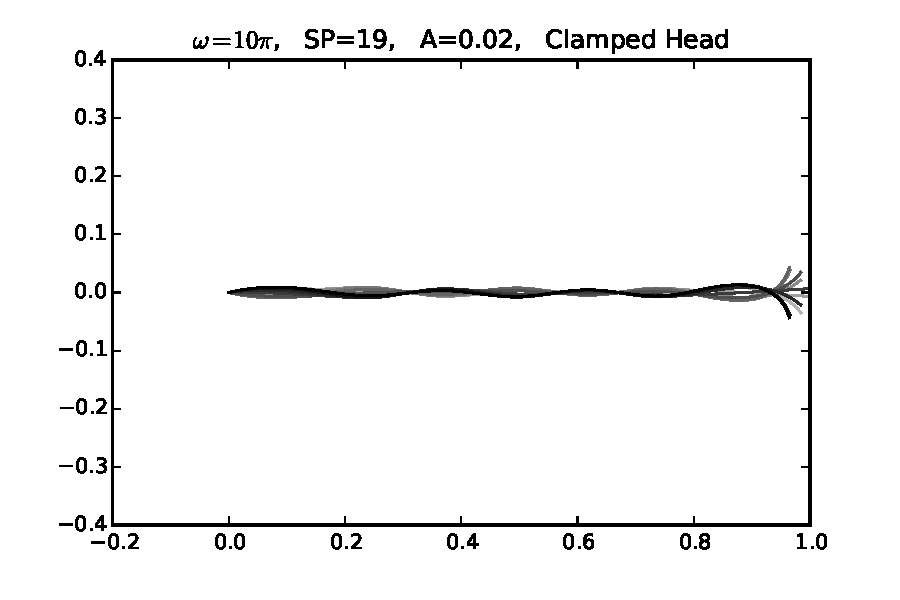
\includegraphics[width=.3\textwidth]{clamped_19_10}
  \label{fig:clamped-head}
\end{figure}


\begin{figure}
  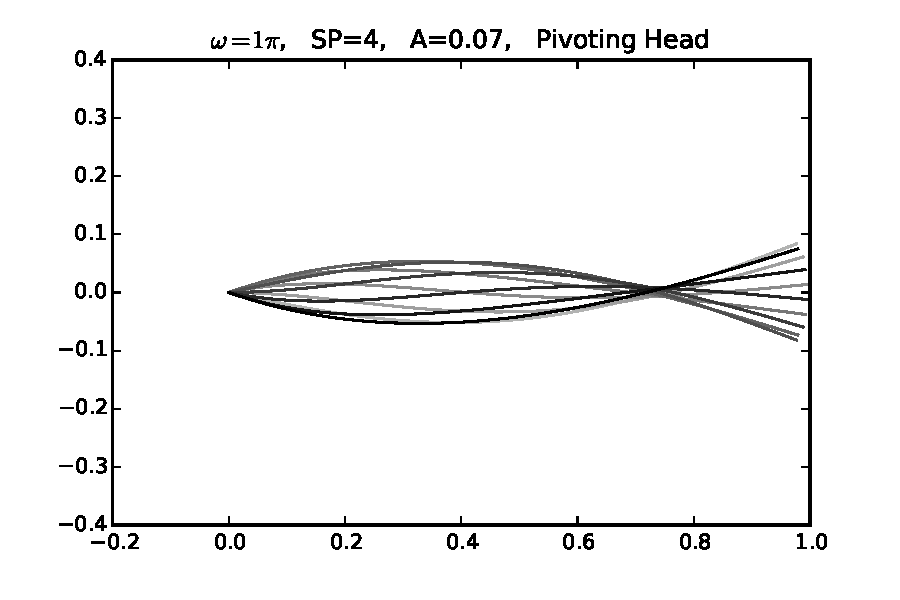
\includegraphics[width=.3\textwidth]{pivoting_4_1}
  \hfill
  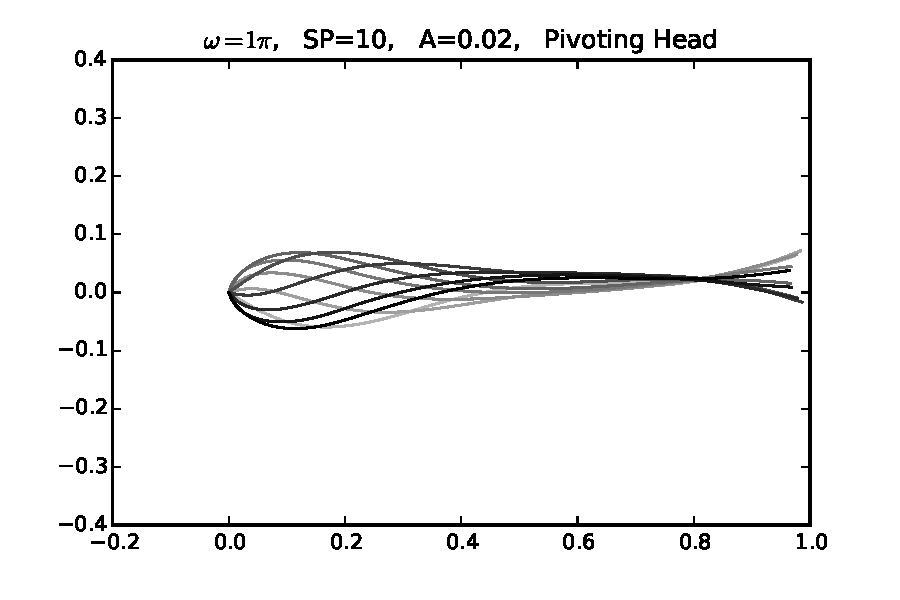
\includegraphics[width=.3\textwidth]{pivoting_10_1}
  \hfill
  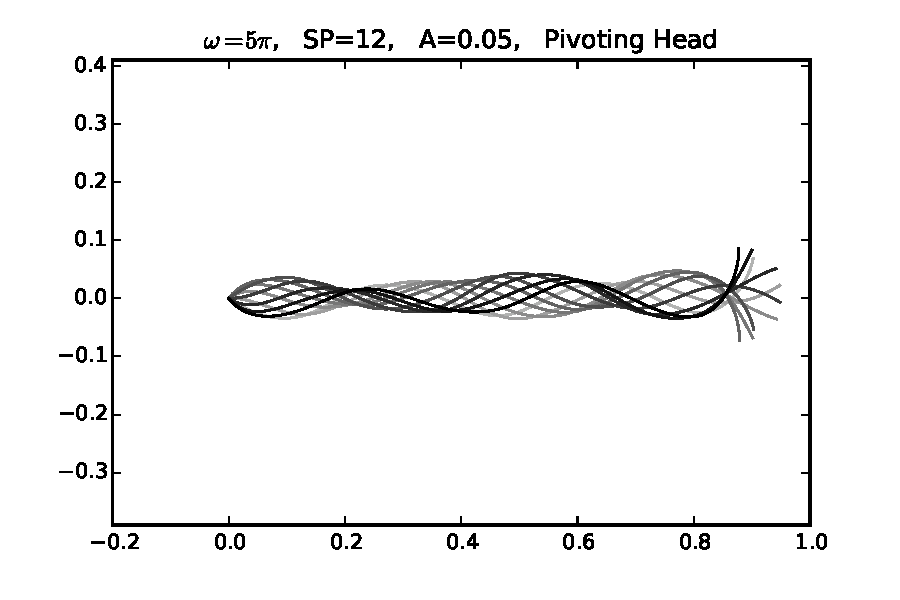
\includegraphics[width=.3\textwidth]{pivoting_12_5}
  
  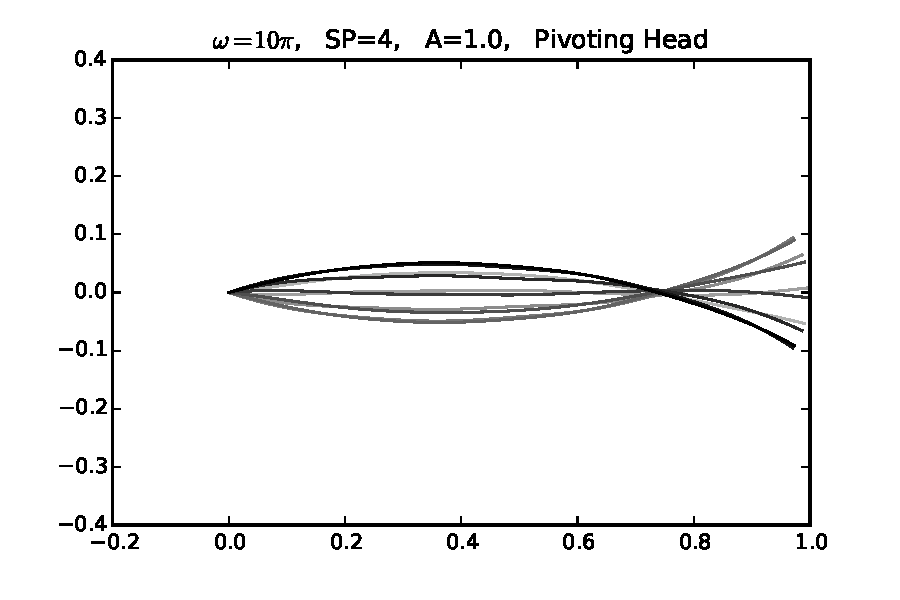
\includegraphics[width=.3\textwidth]{pivoting_4_10}
  \hfill
  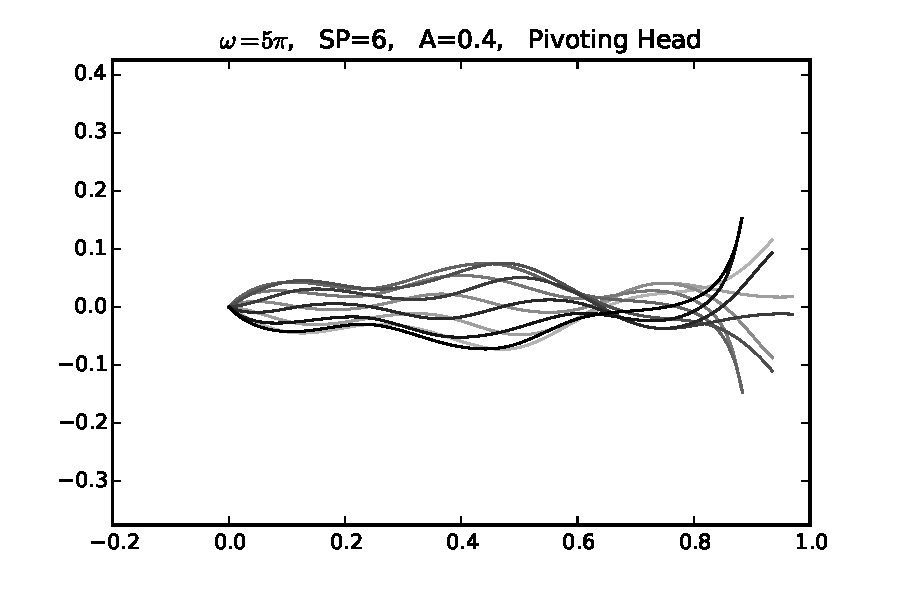
\includegraphics[width=.3\textwidth]{pivoting_6_5}
  \hfill
  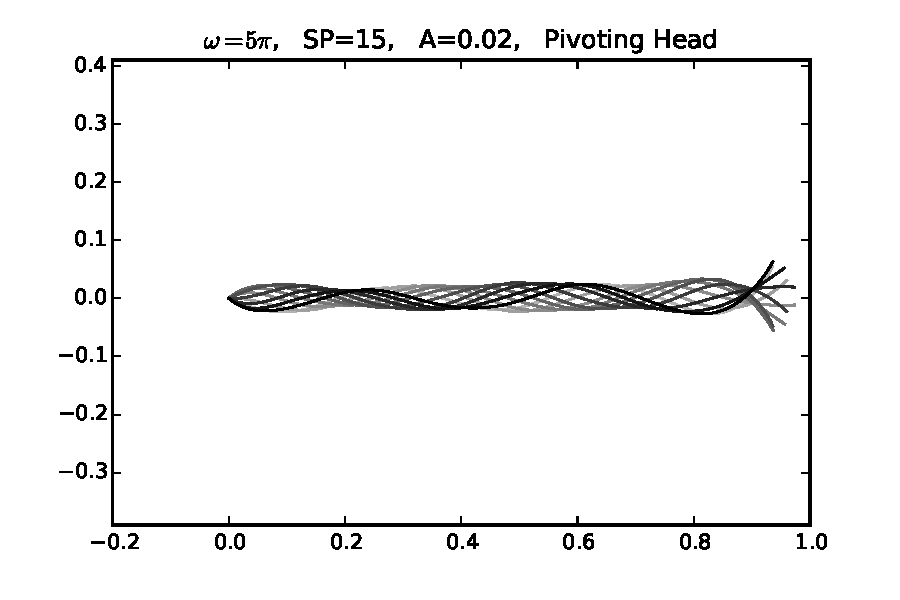
\includegraphics[width=.3\textwidth]{pivoting_15_5}


  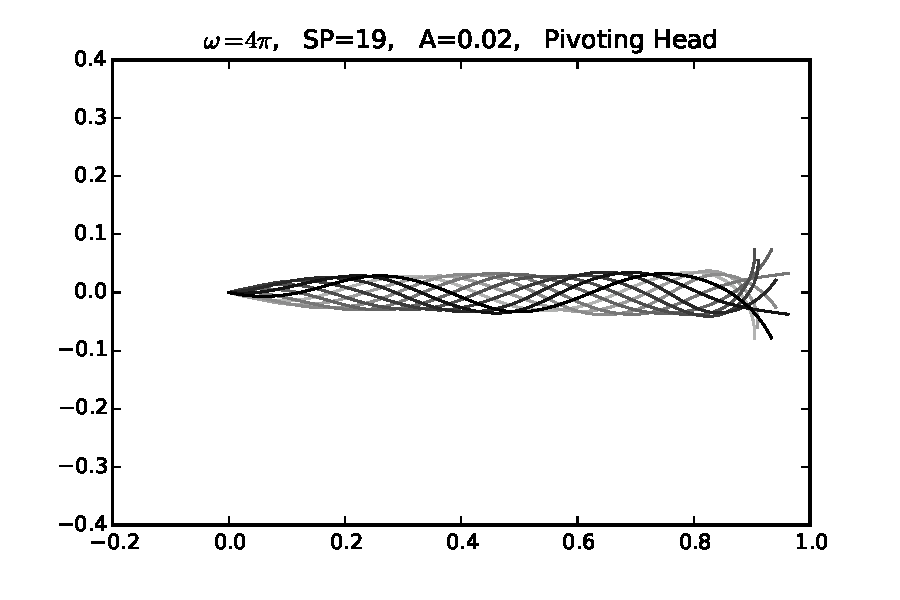
\includegraphics[width=.3\textwidth]{pivoting_19_4}
  \hfill
  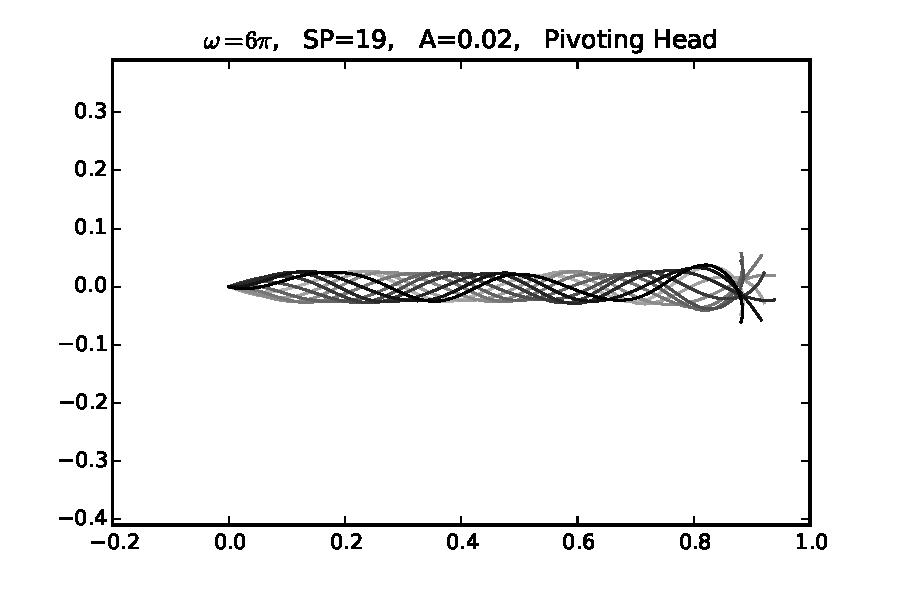
\includegraphics[width=.3\textwidth]{pivoting_19_6}
  \hfill
  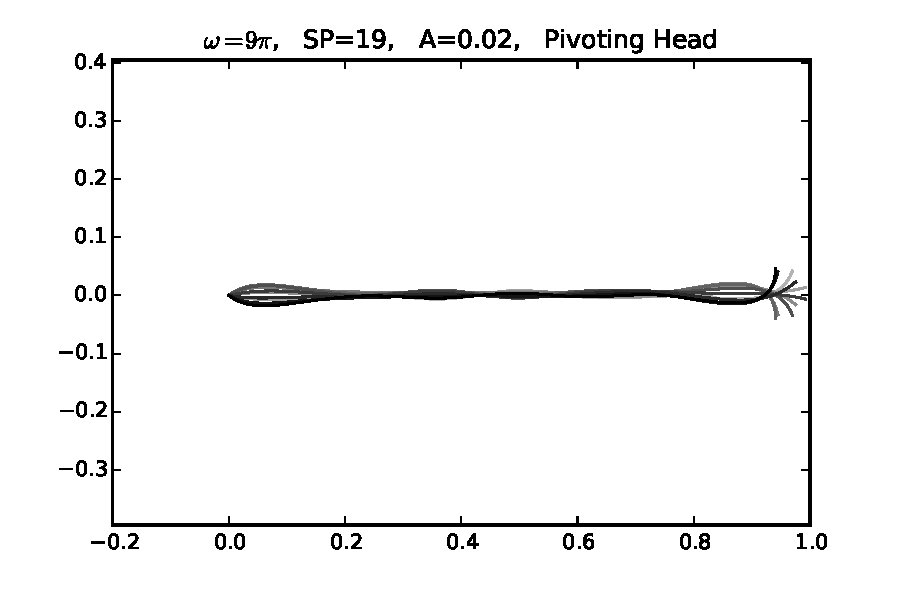
\includegraphics[width=.3\textwidth]{pivoting_19_9}



  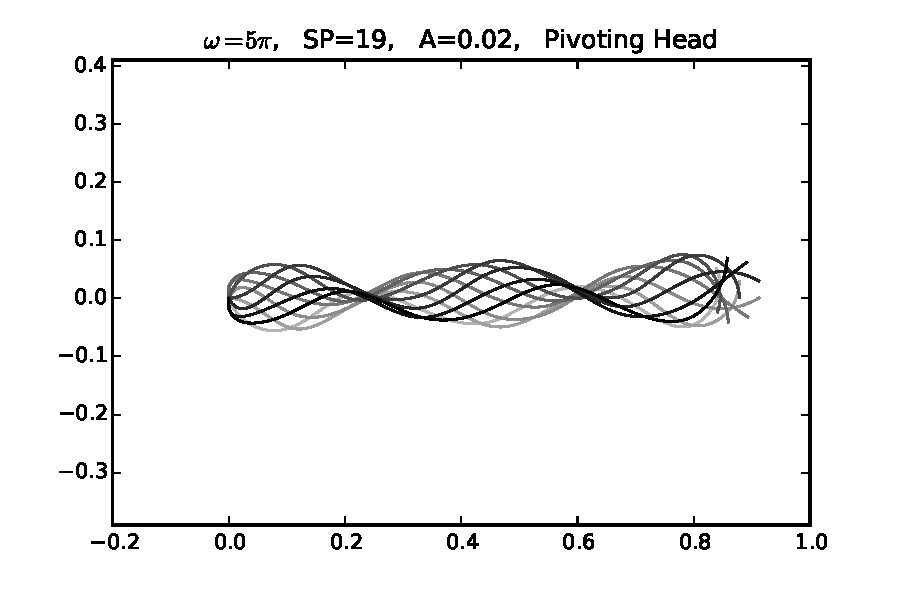
\includegraphics[width=.3\textwidth]{pivoting_19_5}
  \hfill
  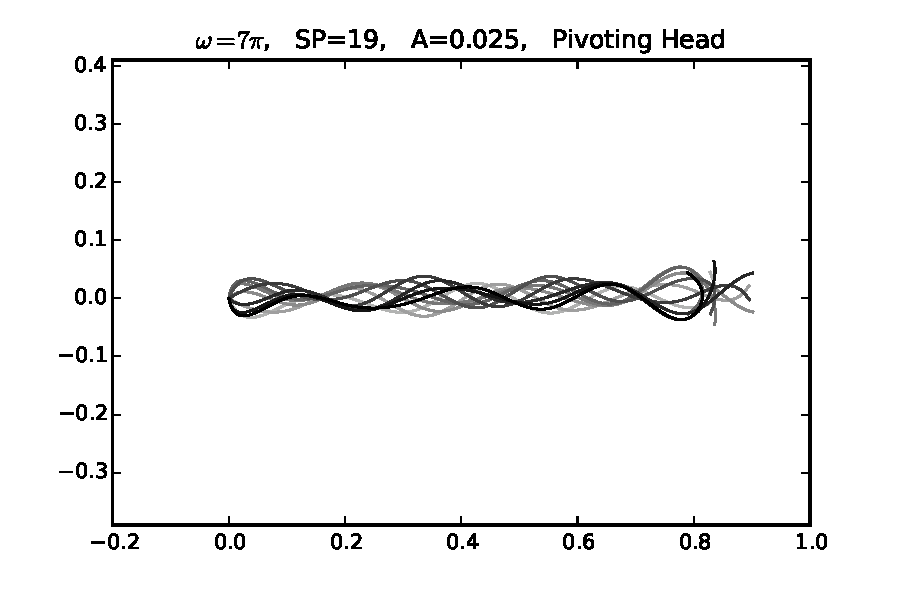
\includegraphics[width=.3\textwidth]{pivoting_19_7}
  \hfill
  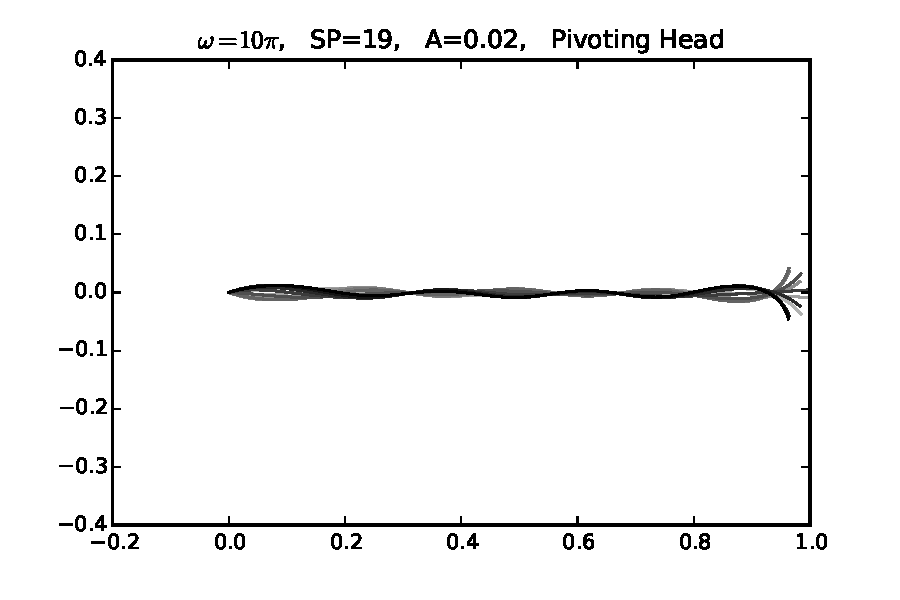
\includegraphics[width=.3\textwidth]{pivoting_19_10}
  \label{fig:pivoting-head}
\end{figure}

In Figure~\ref{fig:clamped-head} and~\ref{fig:pivoting-head} we try to
reproduce the graphs of~\cite{Gadelha2010}, Figure 3. Notice that we
do not observe any nonlinear instability in the clamped case.

\bibliographystyle{plain}
\bibliography{Flagella}

\end{document}

  
  
  
  
  
  
  
  
  